\documentclass[]{article}
\usepackage{graphicx}
\usepackage{subfig}
\usepackage{amsmath}
\usepackage{amsfonts}
\usepackage[margin=1in]{geometry}

\begin{document}
\title{CS689 Final Project:\\ Text Genre Classification in the $n <<p$ Regime}
\author{Sam Anzaroot and David Belanger}
\maketitle
\section{Introduction}

An overwhelming amount of text data becomes available every second. The text comes in chunks corresponding to articles, press releases, blog posts, tweets, etc. These can all be thought of in general terms as `documents'. Suppose you are looking for particular information in a very large collection of documents. A common real world situation is that there are so many documents that the time cost of looking for the information in all of the documents is prohibitive. Many of these documents may be irrelevant, however. You aren't likely to find the latest information on the European economy by looking in the sports section of the Wall Street Journal, but looking in the main section would be fruitful. Here, there are underlying genres for documents given by the section of the newspaper that they appear in. In many settings, annotation of such underlying genres is not available explicitly, and we require automatic methods for discerning the genre of a document. 

Text genre classification can be accomplished by first mapping the document to a numerical feature representation and then using a general-purpose classification algorithm that was trained on labeled examples. 

Certain characteristics of text data make classification particularly challenging, though. These include:
\begin{enumerate}
\item Time has shown that often the best way to embed documents in feature space is to map to a space where each dimension corresponds to a word in the vocabulary. The value in dimension $i$ can be represented, for example, as the frequency of word $i$ appearing in the document. Such representations appear, for example, in state-of-the-art named entity extraction and dependency parsing systems ~\cite{ratinov2009design,nivre2004deterministic}. Due to Zipf's law, the distribution of word usages in most text is extremely heavy-tailed [need a source for this]. Therefore, the dimensionality of the embeddings for documents in feature space can be quite high, in the tens of thousands. 
\item  In a given document, most words in the vocabulary appear 0 times. Given that the feature embedding of documents has a dimension for each word, most dimensions are zero for a particular document. Therefore, features for text data are often extremely sparse. 
\item Data annotation can be expensive. Given the high dimensionality of feature embeddings for documents, we are often in the $n << p$ regime, where $n$ refers to the number of distinct training points and $p$ is the dimensionality of the feature space. 
\end{enumerate}

All three of these factors make classification difficult. Besides classification, additional language processing tasks, which often rely on linear models, svm's, etc. within an inner loop, are challenging because of these data characteristics.  We present experiments  using small amounts of very sparse data for text genre classification in order to help explain general trends and considerations when dealing with data in this difficult regime. 

\section{Background}
\input{Dimensionality}
\subsection{Regularization and Model Sparsity}
	Rather than projecting the data to a lower dimensional subspace, an alternative technique to handle unmanageable input dimensionality is to automatically select which input features are useful and which are not, and only use the relevant ones. In models like logistic regression that place a weight on each input feature, this leads to model sparsity, in that few of the model coefficients are nonzero. This is distinct from data sparsity, in which most of the data matrix is zero. Sparsity of a certain feature by no means suggests that the feature should receive zero weight in the model. For example, in the genre classification example, there may be a word that only in occurs in one-thousandth of the documents, but it is 100\% correlated with the target classification label, and classification should depend on it. 

	In order to achieve model sparsity, one could, for example, find the correlation between target classification labels and each feature and train a model which only considers the most correlated features. The shortcoming of such a technique, however, is that two features that are highly correlated with the labels may also be highly correlated with each other, so that they are no more informative jointly than in isolation ~\cite{tibshirani1996regression}. An alternative technique, which is widely adopted, is to add an $L_1$ regularization term to the training objective function. For example, in a discriminative probabilistic model, which models the conditional probability of the label given the input data, we have the regularized maximum likelihood objective: 
	$$\max_{\theta} \sum_{i = 1}^n log\left(P(y_i | x_i; \theta)\right) + \lambda \lVert \theta \rVert_1$$
Why $L_1$ regularization leads to model sparsity is not immediately obvious. Directly minimizing the number of nonzero coefficients, $\lVert \theta \rVert_0$, would directly reflect our objective. However, this converts the training process to a combinatorial search, which is intractable for high input dimensionality . In some sense, $L_1$ is effective because it is the closest convex regularization term to $L_0$ ~\cite{LectureL1}. Figure \ref{fig:sparsity} is taken from the original paper advocating $L_1$ regularization for linear regression, which is known as the LASSO  ~\cite{tibshirani1996regression}. The axes represent possible values for the coefficients in a two-dimensional regression problem and the filled in square and circle are boundaries for which the $L_1$ and $L_2$ norms of the coefficient vector is less than 1, respectively. Coefficients are chosen to minimize the squared loss between the linear model's prediction and the target values. As a function of the model coefficients, this squared loss takes the form of a quadratic form, so its level sets are ellipses. The level sets are likely to intersect the $L_1$ coefficient square at a corner, yielding only one nonzero coefficient. $L_2$ regularization, on the right, doesn't yield such behavior. 
\begin{center}
\begin{figure}[!ht] 
\centering
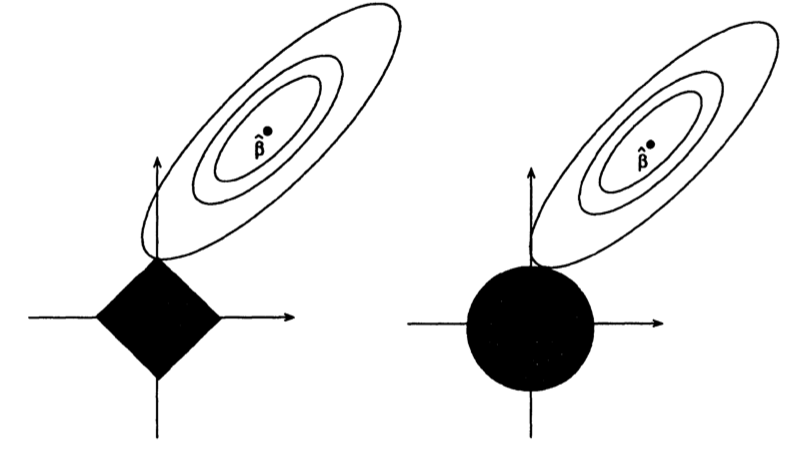
\includegraphics[width=.5\textwidth]{../images/sparsity.png}
\caption{L1 vs. L2 Regularization}
\label{fig:sparsity}
\end{figure}
\end{center}

	A desirable characteristic of model sparsity is that it encourages models that are more interpretable  ~\cite{tibshirani1996regression}. When only a few features are assigned nonzero coefficients, one can deduce which features are relevant for a given prediction problem. When coefficients are diffuse and small but nonzero, interpretation is more difficult. In the context of document genre classification, these sparse feature weights can be quite useful. If it turns out that only a few words are relevant for distinguishing between two genres with high probability, downstream language processing tasks could zoom in on these words. For example, we may have a pipeline where we classify documents into genres and then analyze the sentiment of the documents, conditional on their genres. The genre-specific sentiment model could be based on context features specific to the words that were found to be important when training the classification model. One downside of feature selection by enforcing sparsity is that it won't identify useful, but redundant features ~\cite{LectureL1}. If two features are both useful, but similar, the model will place double weight on one and none on the other. 

	In addition to providing a means for feature selection and model interpretation, regularization is desirable in order to diminish the risk of overfitting, which is a serious concern in the $n << p$ regime. In the formulation above for discriminative probabilistic models, the coefficient $\lambda$ specifies how much to trust the data's inclination for a irregular decision boundary vs. how much to shrink coefficients towards a more simple boundary. Similarly, in support vector machines, the parameter $C$ determines an upper bound on the number of misclassified training points, which controls how irregular the decision boundary can be~\cite[332]{Bishop}.

	It's clear that regularization is desirable in general. In the case of probabilistic models like logistic regression, it's worth considering alternative regularization schemes other that $L_1$, especially if encouraging sparse models is not an objective. A natural alternative is $L_2$ regularization, which is widely used due to its linear gradient. In the case of regularized logistic regression, Andrew Ng produced important theoretical results in 2004 concerning differences between regularization with each. He proved that the ``sample complexity of L1-regularized logistic regression is logarithmic in the number of features." However,  ``the sample complexity of L2-regularized logistic regression is linear in the number of features"  ~\cite{ng2004feature}. Sample complexity is the number of training points necessary to obtain a desired amount of generalization error with a certain probability. The basic intuition for his proof is that the $L_2$ regularized logistic regression objective is invariant to rotations of the training data in feature space, and there exists a pathological rotation such that linear sample size is necessary. $L_1$ regularization doesn't allow such rotations, and further, one can show that it requires logarithmically-many samples. Though these are worst-case asymptotics, Ng show through experiments that  this sample complexity occurs often in practice. Therefore, it seems using $L_1$ regularization for logistic regression in our small-n regime is advisable. For classification settings other than logistic regression, $L_2$ may more desirable in order to maintain a differentiable objective function, however. 

\subsection{Model Selection}
	Now that we have established guiding principles for how to employ dimensionality reduction and regularization in the $n << p$ context we're interested in, we need to discuss more general principles concerning how to choose between various types of models for our genre classification task. In our experiments to follow, we consider 4 principle types of models and a representative for each: probabilistic discriminative (logistic regression), generative (diagonal-gaussian discriminate analysis, i.e. naive Bayes), nonparametric discriminative (support vector machine), and model-free nonparametric (k-nearest neighbors). 

	First, it is important to discuss the distinction between generative and discriminative probabilistic models. Discriminative models, such as conditional random fields, have become popular in recent years because they generally provide superior performance to analogous generative models, in part because they impose fewer assumptions about the underlying data process and because they also provide more flexibility for using non-independent features ~\cite{lafferty2001conditional}. Naive Bayes and logistic regression are generative-discriminative analogues of each other. Both models make decisions based on a linear decision boundary. The hypothesis space for logistic regression is all possible linear boundaries. Naive Bayes is restricted to boundaries that are a subset of this. Therefore, it is not surprising that with large amounts of training data, logistic regression often obtains better test set accuracy ~\cite{jordan2002discriminative}. 	
	
	Based on the asymptotic superiority of discriminative models like logistic regression, it seems we should avoid using something like naive Bayes. However, these asymptotic results only apply in the limit when our training set is quite large.  Further work by Andrew Ng suggests that when we have few training instances relative to the model complexity, generative models may be advisable \cite{jordan2002discriminative}. He argues that as we increase the amount of training data, the generative model obtains a higher asymptotic error, but it approaches this error more quickly than the discriminative model, which approaches its lower error rate more slowly. Therefore, there are two sub-regimes of the amount of training data available, and  the optimal classifier is different  between the two. Since we are studying the context where we don't have much training data, we need to explictly consider which regime we fall in, and not assume the superiority of a discriminative model.
	
	An alternative to both of these models is support vector machines. SVMs are powerful due to their robustness to outliers and elegant modeling of nonlinear decision boundaries through the kernel trick ~\cite{LectureSVM}. SVMs require computing lots of kernel functions between pairs of points. Due to the curse of dimensionality, using any kernel that's a function of $\lVert x_1 - x_2 \rVert$ is inadvisable because this pairwise distance becomes uniform, and thus uninformative, for high-dimensional inputs. A linear kernel, $k(x_1,x_2) = x_1^Tx_2$ does not exhibit this property. It is also extremely efficient to compute for sparse input vectors, because there are few dimensions for which both $x_1$ and $x_2$ are nonzero. Furthermore, the model complexity of an SVM is linear in the number of training points, not the dimensionality of the feature space ~\cite{LectureSVM}. Therefore it seems that SVMs with a linear kernel are a good candidate for classification in the sparse $n << p$ regime. 

	Lastly, another important family of models for classification are nonparametric, model-free methods such as k-nearest neighbors (KNN). Given our argument for the curse of dimensionality, it seems that KNN will perform poorly because points will be uniformly far from each other. In later experiments, we present classification results using KNN in order to understand to what extent we truly are cursed by dimensionality in the feature space describing documents. 

Overall, there is no technique that seems optimal apriori for the type of classification we are doing. Next, we experiment on a real world data set and explore general trends that will inform which type of classification is best, depending on how much data is available and desired characteristics of the model. 

\section{Experiments and Discussion}

For this project we used a post-processed version the Reuters RCV1 dataset ~\cite{lewis2004rcv1}. This dataset is presented as a matrix of the TF-IDF (Term Frequency weighted by importance of term by the logarithm of the number of documents over the number of documents containing the term) values of the words as each feature. For the labels, we selected a target class that had rather high frequency of occurrence, namely C181 (MERGERS/ACQUISITIONS). We subsampled the dataset so as to contain 3000 examples, half of which belong to the target class and half of which belong to any class besides for the target class.
In parallel with the three sections of the paper's background section, we  present experiments and discussion on three themes: dimensionality, regularization and model sparsity, and model selection. 

\subsection{Dimensionality}
%\documentclass[]{article}
%\usepackage{graphicx}
%\usepackage{subfig}
%\usepackage{amsmath}
%\usepackage{amsfonts}
%\usepackage[margin=1in]{geometry}

%\begin{document}


First, it's worth understanding how basic characteristics of our dataset respond to dimensionality reduction.  In figure \ref{fig:PCA_RED} we estimate a 500-dimensional PCA projection (computing more principle components than 500 was intractable on our high-dimensional dataset). Next, we truncate this to a smaller-dimensional projection, and see how aspects of the data scale with projection size. In  \ref{fig:PCA_RED}(a) we compute the total covariance of the first 500 principle components, and then show what fraction of this total covariance is captured as we increase the dimensionality of the projection. We find that the curve grows quite slowly. In order to capture 50\% of the total covariance, we need to use about 150 principle components. In  \ref{fig:PCA_RED}(b) we measure the sparsity (percentage of zero entries) of the projected design matrix. The raw matrix unprojected matrix is 99.6\% sparse. We find that the sparsity increases quite quickly with PCA projection dimension. Therefore, if we want to capture a reasonable amount of the total covariance, we must deal with very sparse data. 

\begin{figure}[!ht]
\centering
\subfloat[Cumulative Cov. vs. dim PCA]{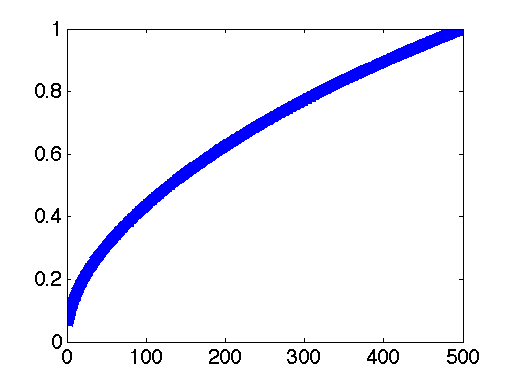
\includegraphics[width=.33\textwidth]{../images/pca_cumsum.png}}
\subfloat[Zoom-in of Cum. Cov. vs. dim PCA]{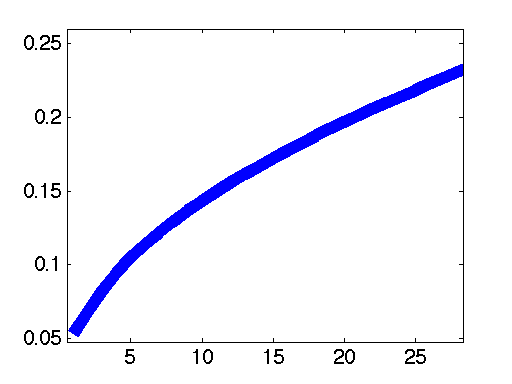
\includegraphics[width=.33\textwidth]{../images/pca_cumsum_zoom.png}}
\subfloat[Data Sparsity vs. dim PCA]{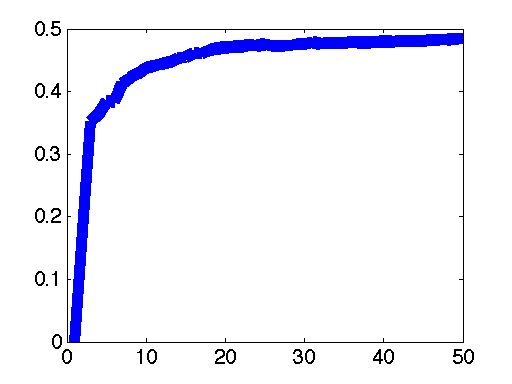
\includegraphics[width=.33\textwidth]{../images/PCAsparsityDensity.png}}
\caption{Characteristics of PCA-reduced data}
\label{fig:PCA_RED}
\end{figure}

Due to this tradeoff between data sparsity and representation of the raw data's variation, it is unclear what the optimal PCA projection dimension is. In figure \ref{fig:pca_acc_vs_proj_dim}, we vary the projection dimension and plot the accuracy of two different classifiers. 

In \ref{fig:pca_acc_vs_proj_dim}(a), we use Naive Bayes, with `add one' smoothing, where a certain number of rows of all ones are added to the design matrix. We choose the number of pseudocounts for these added rows by optimizing classification performance on a development set. Pseudocount optimization is done separately for each PCA dimension, in order to count for the changing sparsity of the data. We find that accuracy peaks when using a 7-dimensional projection. Considering figure  \ref{fig:PCA_RED}, this is unsurprising, because it is around this dimension where the sparsity of the data increases considerably. 

In contrast, in \ref{fig:pca_acc_vs_proj_dim}(b), we use an linear-kernel SVM, which is less sensitive to data sparsity. In contrast with naive Bayes, accuracy stays high when increasing PCA dimension. SVM model complexity scales with the number of training points, not the dimensionality of the input space. Therefore, there is less of a concern when increasing projection dimensionality, and performance increases because in a higher-dimensional projected space, pairwise distances between points are captured with higher fidelity. 

\begin{figure}[!ht]
\centering
\subfloat[Naive Bayes acc. vs. PCA dim]{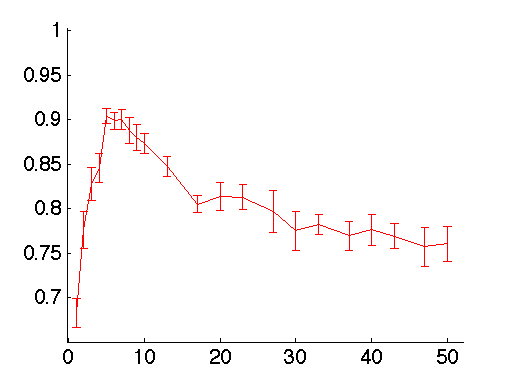
\includegraphics[width=.5\textwidth]{../images/nb_acc_vs_dim_pca_sr.png}}
\subfloat[SVM acc. vs. PCA dim]{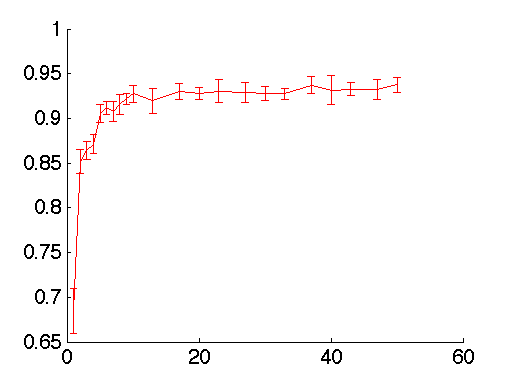
\includegraphics[width=.5\textwidth]{../images/svm_acc_vs_dim_pca_sr.png}}
\caption{Accuracy vs. dim. PCA Projection}
\label{fig:pca_acc_vs_proj_dim}
\end{figure}

Next, we vary the dimensionality of a random projection and compute the 10-fold cross validation accuracy of naive Bayes. We don't experience anything with a distinct peak like we did with PCA, and the overall accuracy isn't as good as with PCA. However, it is important to recognize that we obtain reasonably good classification accuracy using random dimensionality reduction. Estimating the projection matrix for PCA is quite time-intensive, while the random projection matrix can be generated quite easily. Training the naive Bayes model on the reduced data is of course much faster than training on the full 17,000 dimensions. Therefore, for practical situations where a model needs to be trained quickly, random projection and naive Bayes is a good candidate. 

\begin{center}
\begin{figure}[!ht]
\centering
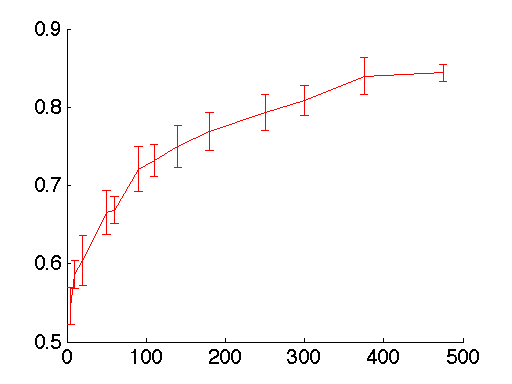
\includegraphics[width=.5\textwidth]{../images/accuracy_vs_dim_randproj.png}
\caption{Naive Bayes Acc. vs. num dim Rand. Projection}
\label{fig:nb_rand_proj}
\end{figure}
\end{center}


	Next, in figure \ref{fig:distance}(a), we explore how the curse of dimensionality affects k-nearest neighbors (KNN) and performing KNN on projected data. We compare 3 scenarios: unprojected 17,000 dimensional data (red), PCA-reduced data (blue), randomly projected data (green). We vary the dimensionality of the projection for the PCA and random projection datasets. We find that  PCA improves KNN over using no projection, even for PCA dimensions as high as 80. 

	The fact that PCA helps may be a consequence of the curse of dimensionality. In higher dimensional spaces, there is less variation among pairwise distances, so classifiers based on pairwise distances may perform worse. To support this claim, in figure ~\ref{fig:distance}(b) we conduct a similar experiment varying PCA dimension, but contrast an the classification accuracy of an SVM with a linear kernel and one with a radial basis kernel. As expected, we find that classification performance with the radial basis kernel decreases with PCA dimension. 

\begin{figure}[!ht]
\centering
\subfloat[Accuracy vs Dim. proj  with KNN]{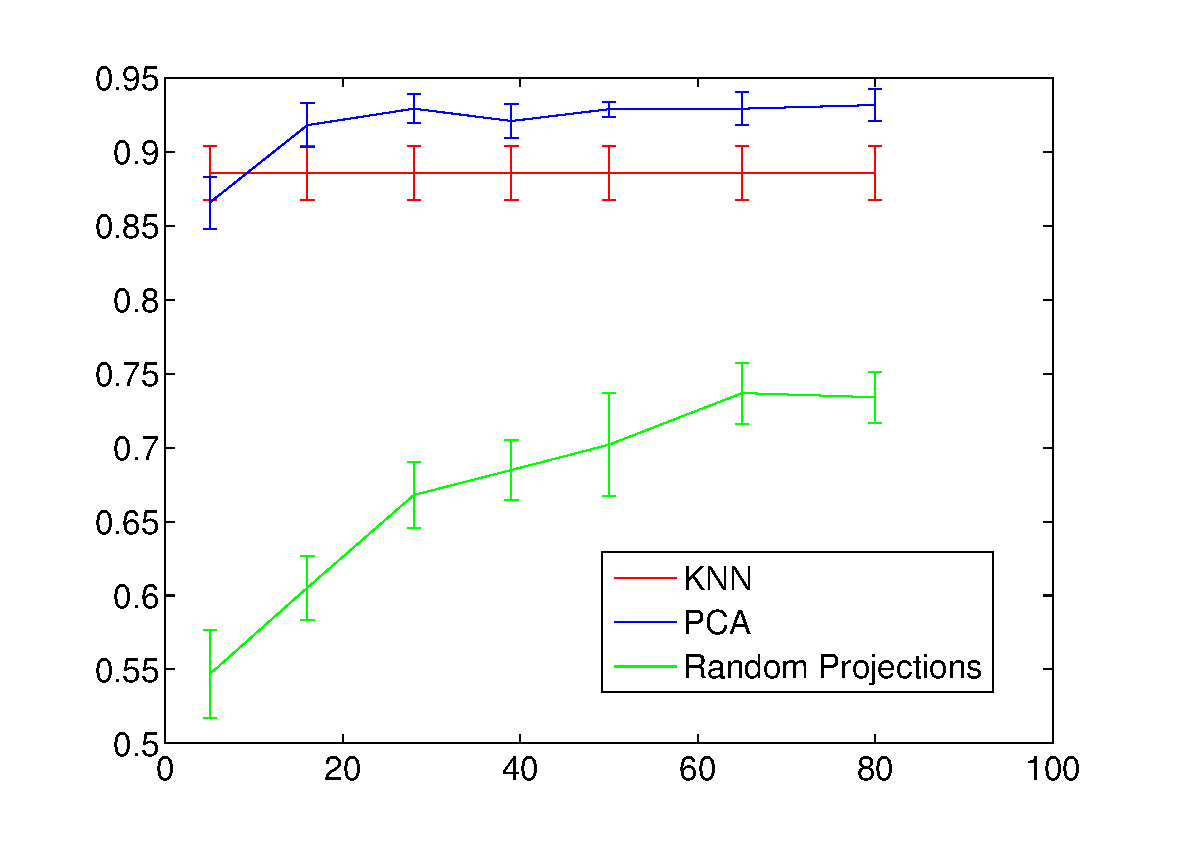
\includegraphics[width=.5\textwidth]{../images/knnVpcaVrproj.eps}}
\subfloat[Accuracy vs Dim. proj  with linear and RBF SVM]{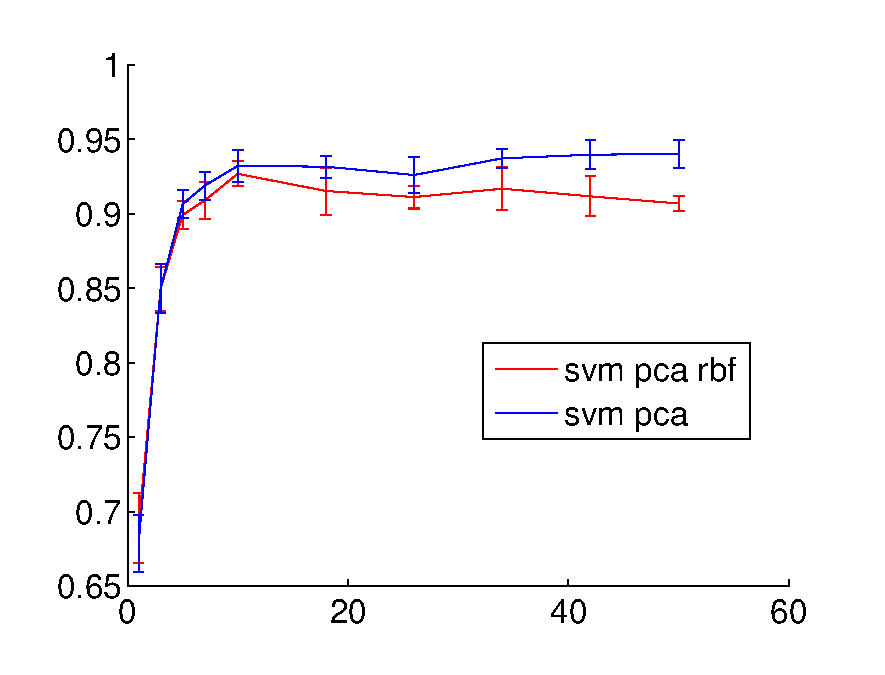
\includegraphics[width=.5\textwidth]{../images/svm_linear_vs_rbf.eps}}
\caption{Curse of Dimensionality and Distance-Based Classification}
\label{fig:distance}
\end{figure}

%\end{document}


\subsection{Regularization and Model Sparsity}
\begin{figure}[!ht]
\centering
\subfloat[L1 regularization]{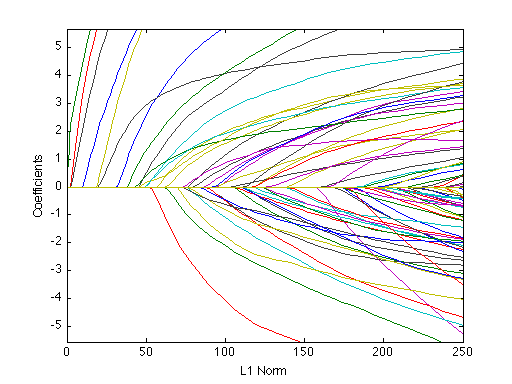
\includegraphics[width=.5\textwidth]{../images/lassoCoeffCurve.png}}
\subfloat[L2 regularization]{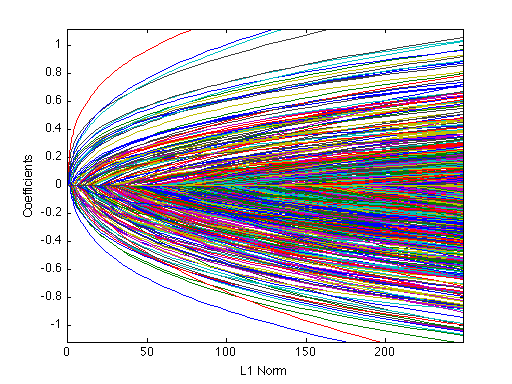
\includegraphics[width=.5\textwidth]{../images/ridgeCoeffCurve.png}}
\caption{Coefficient Paths for Regularized Logistic Regression}
%\label{fig:Coeff_paths}
\end{figure}


\begin{center}
\begin{figure}[!ht]
\centering
\subfloat[Unsorted]{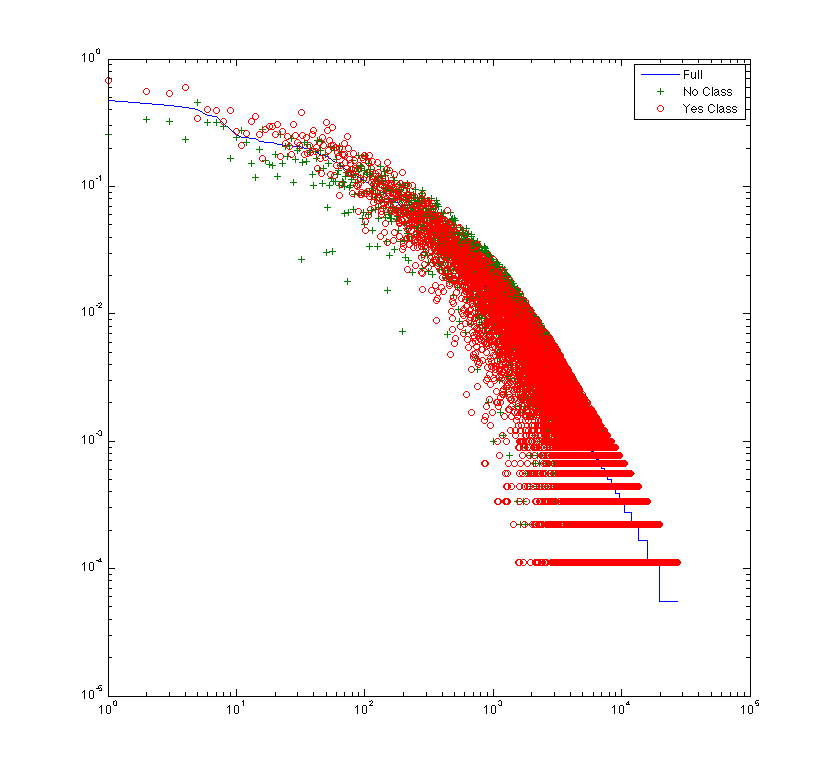
\includegraphics[width=.5\textwidth]{../images/zipfRankedFull.png}}
\subfloat[Sorted]{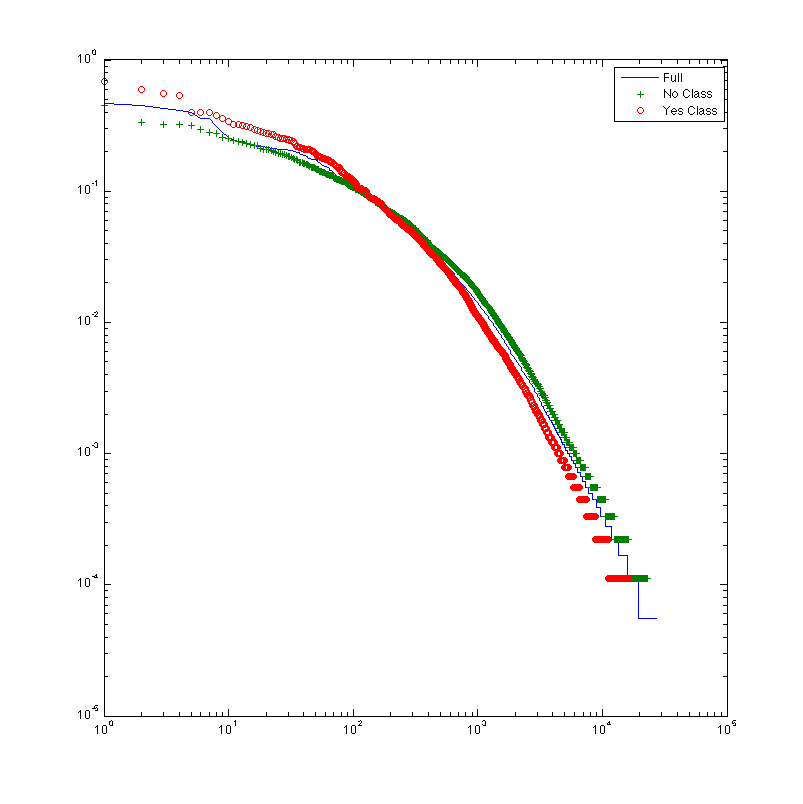
\includegraphics[width=.5\textwidth]{../images/zipfAllSorted.png}}
\caption{Frequency Vs. Rank in full data, target, and other classes}
\label{fig:largecompare}
\end{figure}
\end{center}

\begin{center}
\begin{figure}[!ht]
\centering
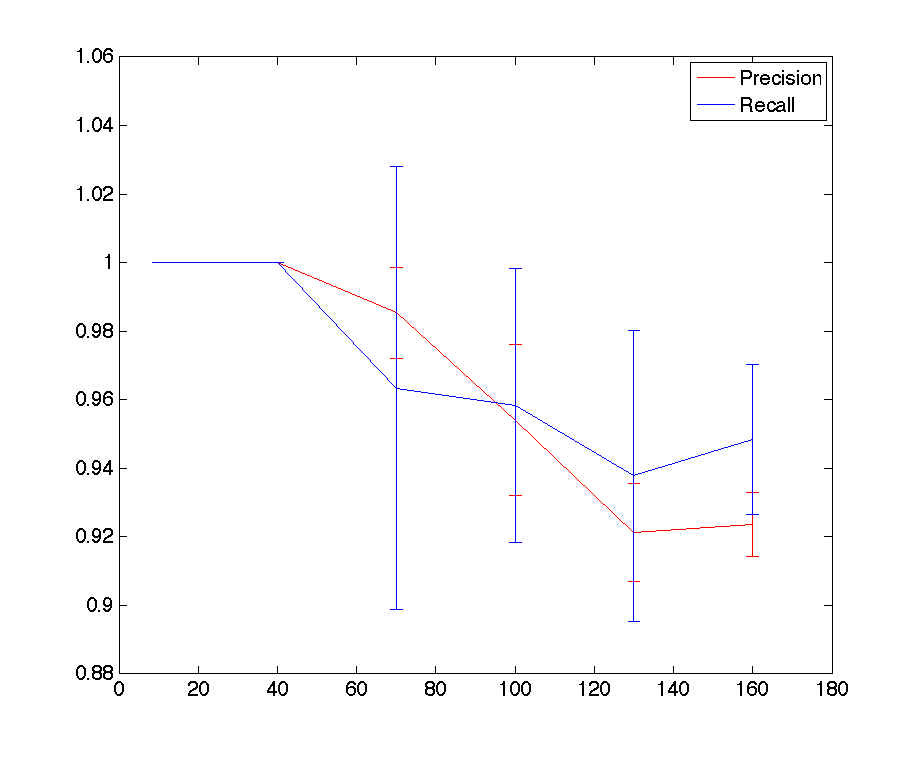
\includegraphics[width=.7\textwidth]{../images/precisionrecallExpansion.png}
\caption{Precision and Recall vs. Number of features selected using LASSO.}
\label{fig:prec recall}
\end{figure}
\end{center}

\begin{center}
\begin{figure}[!ht]
\centering
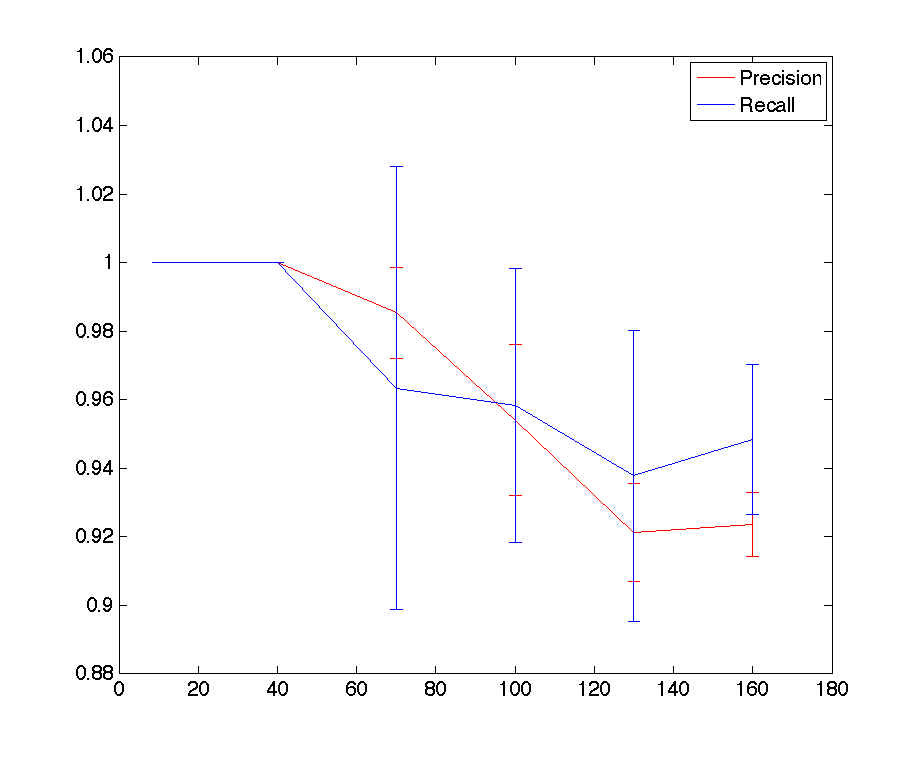
\includegraphics[width=.7\textwidth]{../images/precisionrecallExpansion.png}
\caption{Precision and Recall vs. Number of features selected using LASSO.}
\label{fig:prec recall}
\end{figure}
\end{center}

\begin{tabular}{cccccccccccc}
\hline
Mean&Mean STD&Native Mean&Native STD&Mean Benefit&Benefit STD
\\
\hline
0.9272&0.0099&0.9256&0.0123&-0.0016&0.0069
\end{tabular}


\begin{tabular}{cccccccccccc}
\hline
Precision Mean&Precision STD&Recall Mean&Recall STD
\\
\hline
.7570&0.2913&0.9456&0.1662
\end{tabular}


\begin{tabular}{cccccccccccc}
\hline
Mean Redundant At&Redundant At STD\\
\hline
72.5000&9.6982
\end{tabular}


\subsection{Model Selection}
%\documentclass[]{article}
%\usepackage{graphicx}
%\usepackage{subfig}
%\usepackage{amsmath}
%\usepackage{amsfonts}
%\usepackage[margin=1in]{geometry}

%\begin{document}

Now it's time to actually see how well the various algorithms we have discussed performed on our dataset. In table \ref{tab:AccTable}, we list the performance of various classification algorithms on our dataset. The best performing classifier was an svm that uses the raw data that wasn't reduced in dimensionality. The first 5 rows of the table are all quite comparable in performance, however. 

TODODODODODODO Table with really small number of training examples

\begin{center}
\begin{table}
\begin{tabular}{lccl}
\hline
Name & Mean \% & STD \% & description\\
\hline
svm & 95.0 & 0.8 & svm with linear kernel\\
ridge & 94.0 & 0.2 & $L_2$ regularized logistic regression\\
lasso pca &  94.0 & 0.5 & $L_1$ regularized logistic regression\\
svm pca & 93.3 & 0.2 &  linear kernel svm with 50 dim pca applied first\\
lasso & 92.4 & 0.8 & $L_1$ regularized logistic regression\\
naivebayes smooth pca small & 90.1 & 0.3  & naivebayes smooth with 5-dim. pca\\
naivebayes smooth  & 79.0 & 1.8& naive bayes with `add one' smoothing\\
naivebayes smooth pca  & 77.4 & 0.8 & naivebayes smooth with 50-dim. pca\\
naivebayes smooth rand & 67.0 & 2.8 & naivebayes smooth with 50-dim random projection\\
\end{tabular}
\caption{Classifiers}
\label{tab:Classifiers}
\par
\end{table}
\end{center}


One of our motivating objectives is to find sub-regimes of $n << p$. To do this, we subsampled our training set and varied the size of the reduced set. For each size, we performed 10-fold cross validation. In Figure \ref{fig:largecompareAcc}, we plot the accuracy of the various algorithms as a function of the training set size. We weren't able to find any interesting sub-regimes or crossing points, unfortunately. Perhaps our full dataset was too small to begin with, and interesting sub-regimes would have occurred if we had increased rather than decreased the size of the training data. Another reason that perhaps we don't see any interesting sub-regimes is that classification on our dataset is simply too easy and the performance of many of the classifiers is squeezed into the nineties. 

\begin{center}
\begin{figure}[!ht]
\centering
\subfloat[Accuracy]{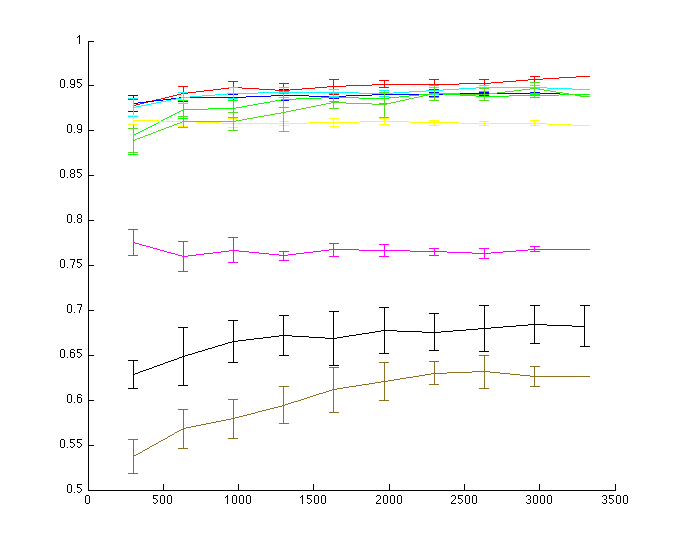
\includegraphics[width=.7\textwidth]{../images/c3.png}}
\subfloat[Legend]{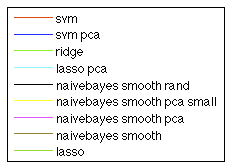
\includegraphics[width=.3\textwidth]{../images/legend.png}}
\caption{Accuracy vs Size of subsampled training data used}
\label{fig:largecompareAcc}
\par
\end{figure}
\end{center}


Overall, one useful a useful outcome of our experiments is that they suggest that sometimes dimensionality reduction is critical when we have little data. To illustrate this phenomenon, in figure \ref{fig:lassoCompare} we vary the size of the training set and compare the accuracy of  $L_1$ regularized logistic regression with and without pca being applied to the data. We find that for extremely small training set sizes, lasso with pca performs substantially better than it does on the raw 17,000 dimensional data. However, as we increase the size of the training set, the performances become comparable. If our dataset had been larger, we would have perhaps identified that the performances cross eventually. 

\begin{center}
\begin{figure}[!ht]
\centering
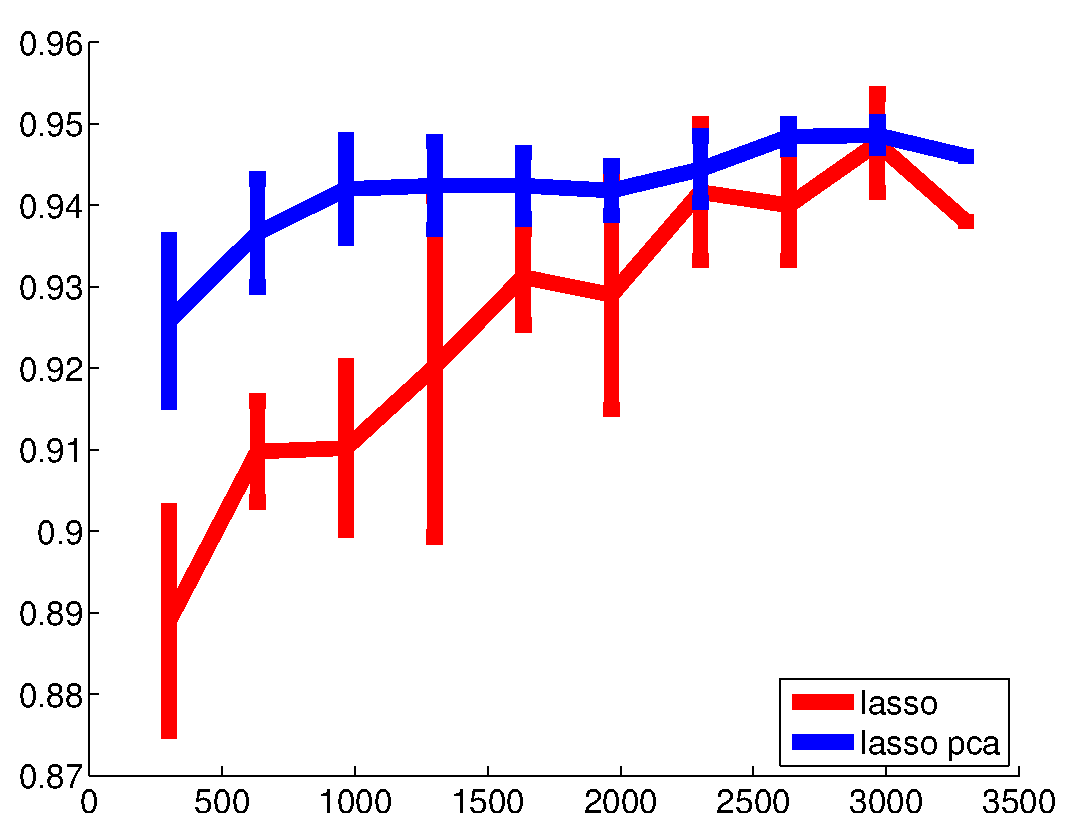
\includegraphics[width=.5\textwidth]{../images/_lasso_lasso_pca_acc.eps}
\caption{Accuracy vs. Train set size}
\par
\label{fig:lassoCompare}
\end{figure}
\end{center}

	In the background section, we discussed an important result due to Ng and Jordan that logistic regression is asymptotically better than naive Bayes, but naive Bayes approaches its higher asymptotic accuracy more quickly ~\ref{jordan2002discriminative}. In figure \ref{fig:LLL}(a), we vary the size of the training set and compare logistic regression with pca and logistic naive Bayes with pca. For this dataset, we are not able to identify a regime of small train set sizes where classification performance for naive Bayes is better. Logistic regression is always superior. One defining characteristic of our dataset, which Ng and Jordan don't account for in their arguments, is the very high level of the data, even after 50-dimensional pca projection (50\% sparse). The number of nonzero observations for each observation is quite low, and thus naive Bayes can not estimate its component-wise Gaussian distributions accurately. Logistic regression makes fewer assumptions about the underlying generative process and consequently less vulnerable to sparsity. 

	We found that dimensionality reduction is important to maintain high classification accuracy for some algorithms in the $n << p$ regime. An additional advantage of it is reduction in time and memory requirements for training. In figure \ref{fig:LLL}(b) we plot the time cost of training a naive Bayes model with pca v.s. a naive Bayes model without pca. We find that the training time for the raw 17,000 dimensional data (red curve) explodes as we increase the training size. Due to the seemingly linear relationship of time vs. train set size for the red curve for most of the train set sizes, its sudden explosion, and the large error bars on the final measurement, it seems like the laptop the experiment was run on became strained and unreliable. When the memory limits of the computer are approached, it suddenly needs to do lots of work to keep things in place, and as a result, runtimes increase tremendously. 


\begin{center}
\begin{figure}[!ht]
\centering
\subfloat[Which of Ng and Jordan's regimes are we in? Accuracy vs. train set size]{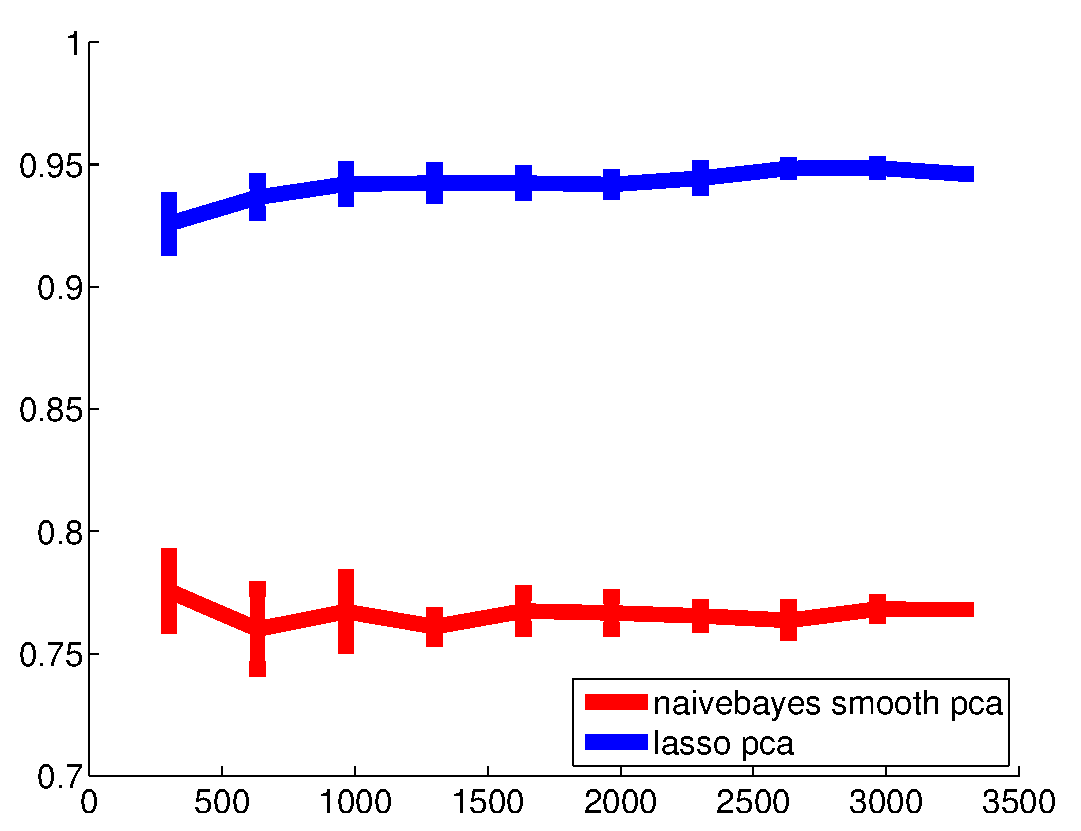
\includegraphics[width=.5\textwidth]{../images/_naivebayes_smooth_pca_lasso_pca_acc.eps}}
\subfloat[NB train time vs. train set size]{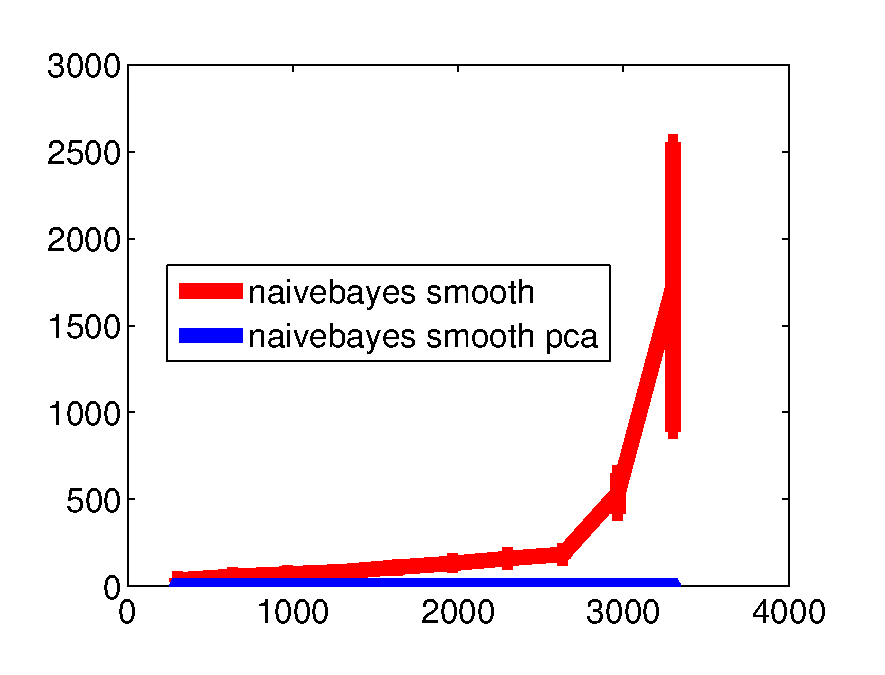
\includegraphics[width=.5\textwidth]{../images/_naivebayes_smooth_naivebayes_smooth_pca_time.eps}}
\label{fig:LLL}
\par
\end{figure}
\end{center}

%\end{document} 



\pagebreak
\bibliographystyle{plain}
\bibliography{citations}

\end{document}

